\chapter{Deployment}
\label{cha:deployment}

\section{Github Organization} % (fold)
\label{sec:github}

This project and all its components belong to a github organization called \texttt{xmlet}\footnote{\href{https://github.com/xmlet}{xmlet Github}}. The aim of that organization is to contain all the related projects to this dissertation. All the generated \ac{API}s are also created as if they belong to this organization. 

\section{Maven} % (fold)
\label{sec:maven}

In order to manage the developed projects a tool for project organization and deployment was used, named Maven. Maven has the goal of organizing a project in many different ways, such as creating a standard of project building and managing project dependencies. Maven was also used to generate documentation and deploying the projects to a central code repository, Maven Central Repository\footnote{\href{https://search.maven.org/}{Maven Central Repository}}. All the releases of projects belonging to the \texttt{xmlet} Github organization can be found under the groupId, \href{https://search.maven.org/#search%7Cga%7C1%7Ccom.github.xmlet}{com.github.xmlet}. 

\section{Sonarcloud} % (fold)
\label{sec:sonarcloud}

Code quality and its various implications such as security, low performance and bugs should always be an important issue to a programmer. With that in mind all the projects contained in the \texttt{xmlet} solution were evaluated in various metrics and the results made public for consultation. This way, either future users of those projects or developers trying to improve the projects can check the metrics as another way of validating the quality of the produced code. The tool to perform this evaluation was Sonarcloud\footnote{\href{https://sonarcloud.io/organizations/xmlet/projects}{Sonarcloud xmlet page}}, which provides free of charge evaluations and stores the results which are available for everyone. Sonarcloud also provides an \ac{API} to show badges that allow to inform users of different metrics regarding a project. Those badges are presented in the \texttt{xmlet} modules Github pages, as shown in Figure \ref{project_badges}.

\begin{figure}[h]
	\centering
	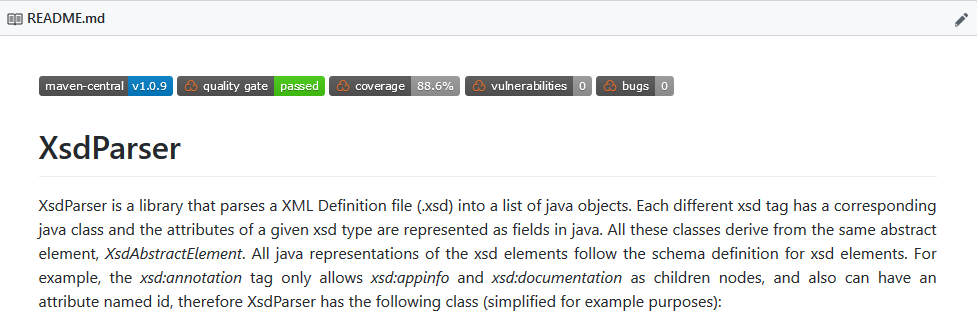
\includegraphics[width=1\textwidth]{badges}
	\caption{XsdParser Github badges}
	\label{project_badges}
\end{figure}

\section{Testing metrics} % (fold)
\label{sec:testingmetrics}

To assert the performance of the \texttt{xmlet} solution we used the \ac{HTML}5 use case to compare it against the J2html (Section \ref{sec:j2html}) and Apache Velocity (Section \ref{sec:apachevelocity}), presented earlier. This two libraries have a difference that is crucial when dealing with performance, J2html doesn't indent the generated \ac{HTML} while Apache Velocity does it. In order to perform a fair comparison between solutions two Visitors were used with the \ac{HTML}5 solution, one that indents the \ac{HTML} to compare it with Velocity and other that doesn't indent it to compare it to J2html. The computer used to perform all the tests present in this section has the following specs:

Processor: Intel Core i3-3217U 1.80GHz\\
RAM: 4GB

\noindent
The tests that are presented below consist in a simple \ac{HTML} document, with a table and a variable amount of table entries as shown in Listing \ref{lst:testhtml}. 

\lstset{language=html}

\begin{minipage}{\linewidth}
\begin{lstlisting}[caption={Test HTML}, label={lst:testhtml}]
<html>
    <body>
        <table>
            <tr>
                <th>
                    Title
                </th>
            </tr>
            
            <!-- Repeated based on the number of elements -->
            <tr>
                <td>
                    ElemX
                </td>
            </tr>
        </table>
    </body>
</html>
\end{lstlisting}
\end{minipage}

The textual elements to feature in the table data rows are stored in a data structure and each solution should iterate that structure when generating the expected \ac{HTML}. To assert which solution is the fastest each one of them will generate the same code and we will verify the number of iterations that are possible to perform in a unit of time. To achieve this objective we will use \ac{JMH}\footnote{\href{http://openjdk.java.net/projects/code-tools/jmh/}{JMH Website}}, which is a tool used for benchmarking. The values gathered are result of the mean values of 8 testing iterations after 12 iterations of warm up. 

\newpage

Generating a table with 10 elements: 

\begin{center}
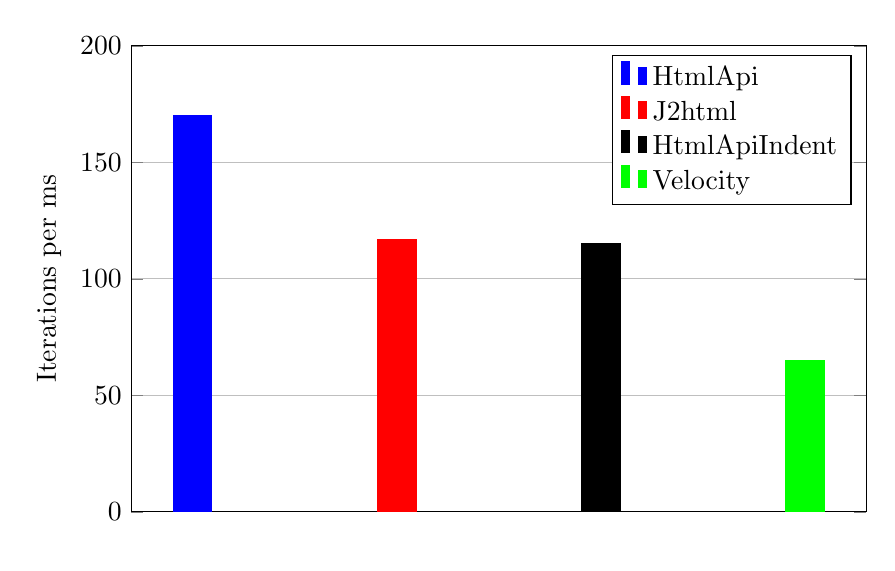
\begin{tikzpicture}
    \begin{axis}[
        width  = 0.9*\textwidth,
        height = 7.5cm,
        major x tick style = transparent,
        ybar=2*\pgflinewidth,
        bar width=14pt,
        ymajorgrids = true,
        ylabel = {Iterations per ms},
		symbolic x coords={HtmlApi, J2Html, HtmlApiIndent, Velocity},
        xticklabels = {},
        scaled y ticks = false,
        enlarge x limits=0.25,
        ymin=0,
        ymax=200,
        legend cell align=left,]
        
        \addplot[style={blue,fill=blue,mark=none}]
            coordinates {(HtmlApi, 170)};
        \addplot[style={red,fill=red,mark=none}]
             coordinates {(J2Html, 117)};
        \addplot[style={black,fill=black,mark=none}]
             coordinates {(HtmlApiIndent, 115)};
		\addplot[style={green,fill=green,mark=none}]
             coordinates {(Velocity, 65)};

        \legend{HtmlApi, J2html, HtmlApiIndent, Velocity}
    \end{axis}
\end{tikzpicture}
\end{center}

Generating a table with 100 elements: 

\begin{center}
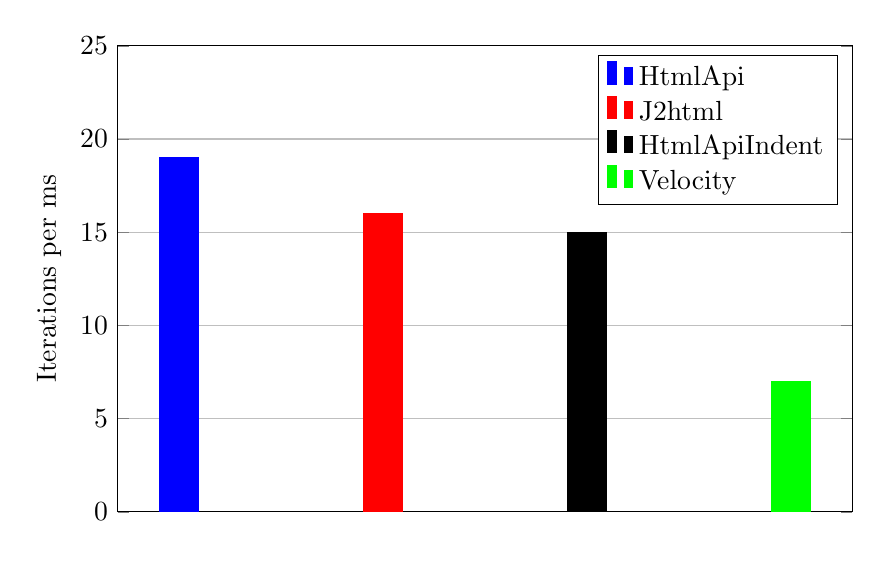
\begin{tikzpicture}
    \begin{axis}[
        width  = 0.9*\textwidth,
        height = 7.5cm,
        major x tick style = transparent,
        ybar=2*\pgflinewidth,
        bar width=14pt,
        ymajorgrids = true,
        ylabel = {Iterations per ms},
		symbolic x coords={HtmlApi, J2Html, HtmlApiIndent, Velocity},
        xticklabels = {},
        scaled y ticks = false,
        enlarge x limits=0.25,
        ymin=0,
        ymax=25,
        legend cell align=left,]
        
		\addplot[style={blue,fill=blue,mark=none}]
            coordinates {(HtmlApi, 19)};
        \addplot[style={red,fill=red,mark=none}]
             coordinates {(J2Html, 16)};
        \addplot[style={black,fill=black,mark=none}]
             coordinates {(HtmlApiIndent, 15)};
		\addplot[style={green,fill=green,mark=none}]
             coordinates {(Velocity, 7)};

        \legend{HtmlApi, J2html, HtmlApiIndent, Velocity}
    \end{axis}
\end{tikzpicture}
\end{center}

%BenchmarkMain.htmlApiBenchmarkTableNoIndentation              10  thrpt    8  171915$712 ± 1822$305  ops/s
%BenchmarkMain.htmlApiBenchmarkTableNoIndentation             100  thrpt    8   19760$504 ±  560$734  ops/s
%BenchmarkMain.htmlApiBenchmarkTableNoIndentation            1000  thrpt    8    2008$911 ±   28$104  ops/s
%BenchmarkMain.htmlApiBenchmarkTableNoIndentation           10000  thrpt    8     241$873 ±    3$225  ops/s
%BenchmarkMain.htmlApiBenchmarkTableNoIndentation          100000  thrpt    8      22$169 ±    0$652  ops/s
%BenchmarkMain.j2htmlBenchmark                                 10  thrpt    8  114187$062 ± 1852$635  ops/s
%BenchmarkMain.j2htmlBenchmark                                100  thrpt    8   16572$066 ±  174$217  ops/s
%BenchmarkMain.j2htmlBenchmark                               1000  thrpt    8    1787$735 ±   27$369  ops/s
%BenchmarkMain.j2htmlBenchmark                              10000  thrpt    8     194$768 ±    2$181  ops/s
%BenchmarkMain.j2htmlBenchmark                             100000  thrpt    8      17$708 ±    0$793  ops/s

Generating a table with 1.000 elements: 

\begin{center}
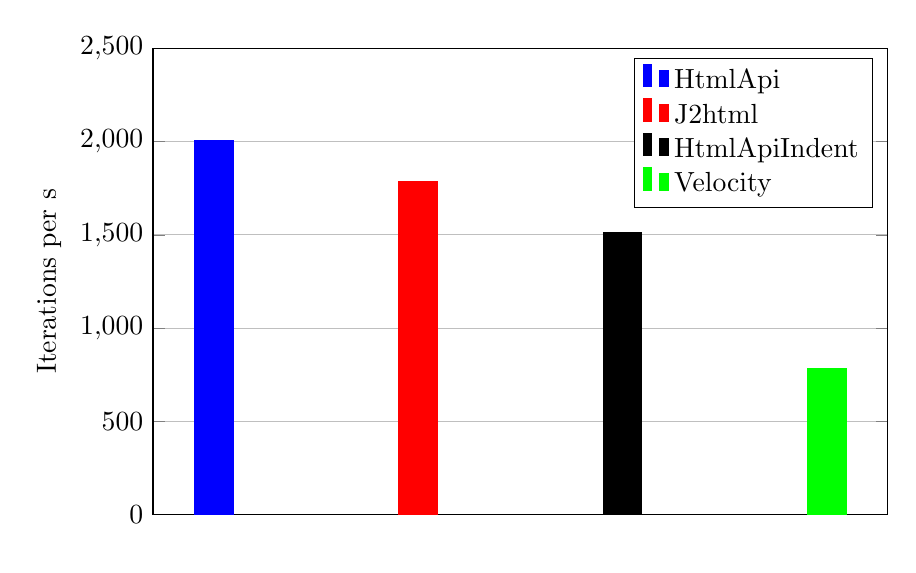
\begin{tikzpicture}
    \begin{axis}[
        width  = 0.9*\textwidth,
        height = 7.5cm,
        major x tick style = transparent,
        ybar=2*\pgflinewidth,
        bar width=14pt,
        ymajorgrids = true,
        ylabel = {Iterations per s},
		symbolic x coords={HtmlApi, J2Html, HtmlApiIndent, Velocity},
        xticklabels = {},
        scaled y ticks = false,
        enlarge x limits=0.25,
        ymin=0,
        ymax=2500,
        legend cell align=left,
    ]
		\addplot[style={blue,fill=blue,mark=none}]
            coordinates {(HtmlApi, 2008)};
        \addplot[style={red,fill=red,mark=none}]
             coordinates {(J2Html, 1787)};
        \addplot[style={black,fill=black,mark=none}]
             coordinates {(HtmlApiIndent, 1515)};
		\addplot[style={green,fill=green,mark=none}]
             coordinates {(Velocity, 781)};   

        \legend{HtmlApi, J2html, HtmlApiIndent, Velocity}
    \end{axis}
\end{tikzpicture}
\end{center}

Generating a table with 10.000 elements: 

\begin{center}
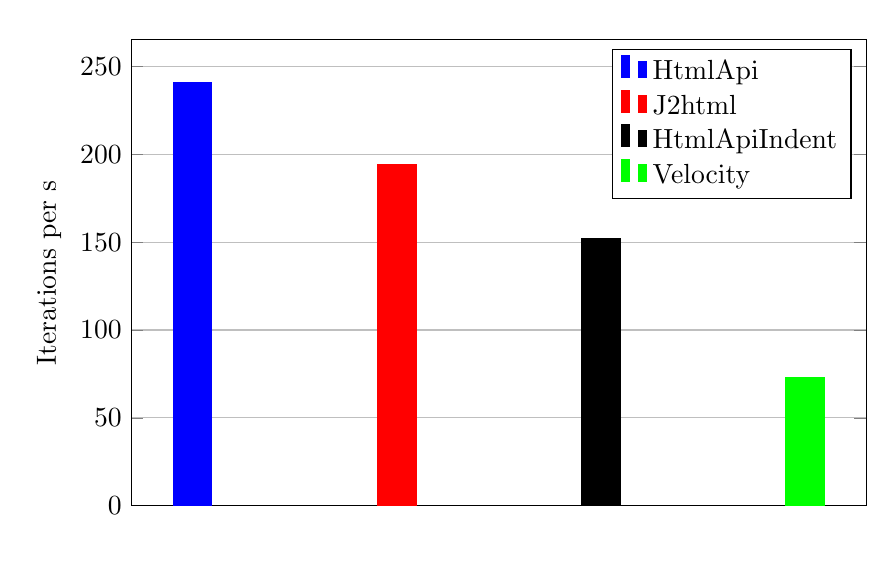
\begin{tikzpicture}
    \begin{axis}[
        width  = 0.9*\textwidth,
        height = 7.5cm,
        major x tick style = transparent,
        ybar=2*\pgflinewidth,
        bar width=14pt,
        ymajorgrids = true,
        ylabel = {Iterations per s},
		symbolic x coords={HtmlApi, J2Html, HtmlApiIndent, Velocity},
        xticklabels = {},
        scaled y ticks = false,
        enlarge x limits=0.25,
        ymin=0,
        legend cell align=left,]

		\addplot[style={blue,fill=blue,mark=none}]
            coordinates {(HtmlApi, 241)};
        \addplot[style={red,fill=red,mark=none}]
             coordinates {(J2Html, 194)};
        \addplot[style={black,fill=black,mark=none}]
             coordinates {(HtmlApiIndent, 152)};
		\addplot[style={green,fill=green,mark=none}]
             coordinates {(Velocity, 73)};      
             
        \legend{HtmlApi, J2html, HtmlApiIndent, Velocity}
    \end{axis}
\end{tikzpicture}
\end{center}

%Benchmark                            (elementCount)   Mode  Cnt       Score      Error  Units
%BenchmarkMain.htmlApiBenchmarkTable              10  thrpt    8  115288$479 ± 3165$561  ops/s
%BenchmarkMain.htmlApiBenchmarkTable             100  thrpt    8   15434$480 ±  214$479  ops/s
%BenchmarkMain.htmlApiBenchmarkTable            1000  thrpt    8    1515$100 ±   35$935  ops/s
%BenchmarkMain.htmlApiBenchmarkTable           10000  thrpt    8     152$280 ±    1$940  ops/s
%BenchmarkMain.velocityBenchmark                  10  thrpt    8   65338$534 ± 1238$090  ops/s
%BenchmarkMain.velocityBenchmark                 100  thrpt    8    7586$455 ±  192$201  ops/s
%BenchmarkMain.velocityBenchmark                1000  thrpt    8     781$837 ±   16$412  ops/s
%BenchmarkMain.velocityBenchmark               10000  thrpt    8      73$138 ±    3$134  ops/s

\noindent
As we can see by the presented results the HtmlApi outperforms the other solutions, either with few elements or with a large number of elements. A second benchmark was performed by using a preexisting project that compares 10 different template engines. The spring-comparing-template-engines project\footnote{\href{https://github.com/jreijn/spring-comparing-template-engines}{Template Engines Benchmark}} uses a tomcat server to launch a WebApi based on Java Spring\footnote{\href{https://spring.io/}{Java Spring}} which can be queried using the name of the template engine, i.e. if we want to use the \ac{API} with the Apache Velocity template engine we  can query http://localhost:8080/velocity. The \ac{API} always returns the same \ac{HTML} page, the only difference is the template engine that was used to generate that page. In order to use this benchmark to also test the HtmlApi another entry was added in the project configuration to make it as if HtmlApi was a template engine solution. 

\noindent
After launching the tomcat server running the Java Spring WebApi another tool is needed to perform the benchmark, ApacheBench\footnote{\href{https://httpd.apache.org/docs/2.4/programs/ab.html}{ApacheBench}}. This tool is used to flood a given \ac{URL} with requests and measures how much time it took for the server to respond to those requests. The values presented below are the result of a single iteration after running two warm up iterations. Multiple variants were used to test the template engines and the HtmlApi solution. The presented results are obtained after running the specified benchmark and \textit{removing} the Spring overhead. The Spring overhead is obtained by performing the respective benchmark to a route that simply returns a empty string.

\newpage

10.000 requests, 10 threads, Spring overhead 1.031 seconds:

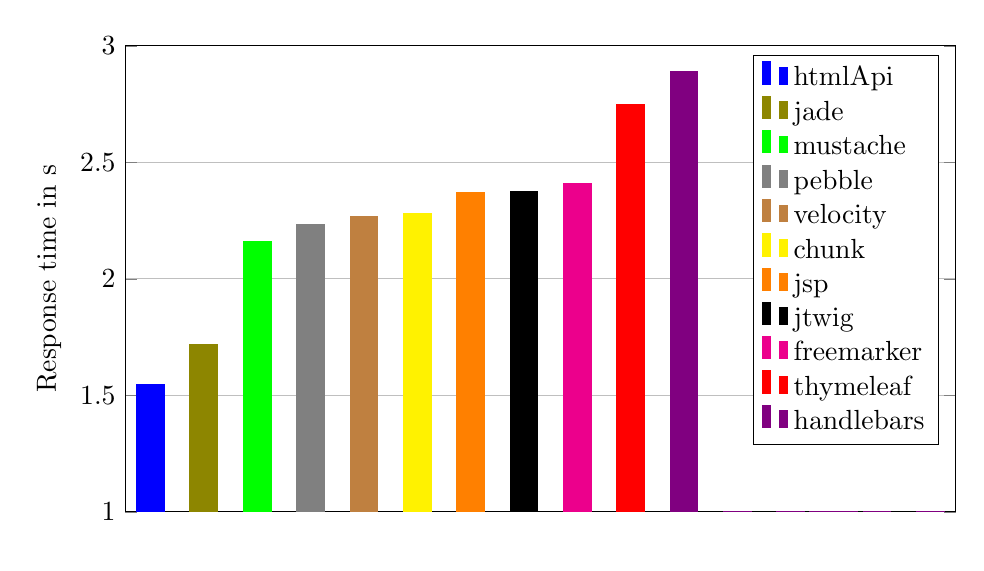
\begin{tikzpicture}
    \begin{axis}[
        width  = 1*\textwidth,
        height = 7.5cm,
        major x tick style = transparent,
        ybar=1*\pgflinewidth,
        bar width=10pt,
        ymajorgrids = true,
        ylabel = {Response time in s},
		symbolic x coords={htmlApi,jade,mustache,pebble,velocity,chunk,jsp,jtwig,freemarker,thymeleaf,handlebars, dummy1, dummy2, dummy3},
        %xtick = data,
        xticklabels = {},
        scaled y ticks = false,
        enlarge x limits=0.8,
        ymin=1,
        ymax=3,
        legend cell align=left,]
                
        \addplot[style={blue,fill=blue,mark=none}]
            coordinates {(htmlApi, 1.547)};
        \addplot[style={olive,fill=olive,mark=none}]
            coordinates {(jade, 1.719)};
        \addplot[style={green,fill=green,mark=none}]
            coordinates {(mustache, 2.158)};
        \addplot[style={gray,fill=gray,mark=none}]
            coordinates {(pebble, 2.235)};
        \addplot[style={brown,fill=brown,mark=none}]
            coordinates {(velocity, 2.266)};
        \addplot[style={yellow,fill=yellow,mark=none}]
            coordinates {(chunk, 2.282)};
        \addplot[style={orange,fill=orange,mark=none}]
            coordinates {(jsp, 2.371)};
        \addplot[style={black,fill=black,mark=none}]
            coordinates {(jtwig, 2.375)};
        \addplot[style={magenta,fill=magenta,mark=none}]
            coordinates {(freemarker, 2.407)};
        \addplot[style={red,fill=red,mark=none}]
            coordinates {(thymeleaf, 2.750)};
        \addplot[style={violet,fill=violet,mark=none}]
            coordinates {(handlebars, 2.891)};
        \addplot[style={violet,fill=violet,mark=none}]
            coordinates {(dummy1, 0)};
        \addplot[style={violet,fill=violet,mark=none}]
            coordinates {(dummy2, 0)};
        \addplot[style={violet,fill=violet,mark=none}]
            coordinates {(dummy3, 0)};
        \addplot[style={violet,fill=violet,mark=none}]
            coordinates {(dummy1, 0)};
        \addplot[style={violet,fill=violet,mark=none}]
            coordinates {(dummy2, 0)};
        \addplot[style={violet,fill=violet,mark=none}]
            coordinates {(dummy3, 0)};
        \legend{htmlApi, jade, mustache, pebble, velocity, chunk, jsp, jtwig, freemarker, thymeleaf, handlebars}
    \end{axis}
\end{tikzpicture}

30.000 requests, 10 threads, Spring overhead 3.285 seconds:

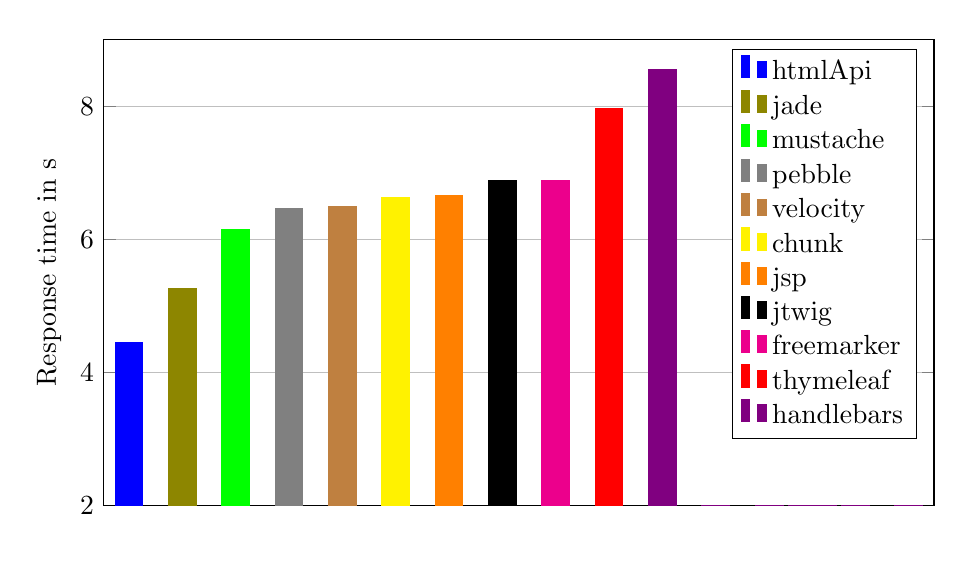
\begin{tikzpicture}
    \begin{axis}[
        width  = 1*\textwidth,
        height = 7.5cm,
        major x tick style = transparent,
        ybar=1*\pgflinewidth,
        bar width=10pt,
        ymajorgrids = true,
        ylabel = {Response time in s},
		symbolic x coords={htmlApi,jade,mustache,pebble,velocity,chunk,jsp,jtwig,freemarker,thymeleaf,handlebars, dummy1, dummy2, dummy3},
        %xtick = data,
        xticklabels = {},
        scaled y ticks = false,
        enlarge x limits=0.8,
        ymin=2,
        ymax=9,
        legend cell align=left,]
                
        \addplot[style={blue,fill=blue,mark=none}]
            coordinates {(htmlApi, 4.450)};
        \addplot[style={olive,fill=olive,mark=none}]
            coordinates {(jade, 5.262)};
        \addplot[style={green,fill=green,mark=none}]
            coordinates {(mustache, 6.153)};
        \addplot[style={gray,fill=gray,mark=none}]
            coordinates {(pebble, 6.465)};
        \addplot[style={brown,fill=brown,mark=none}]
            coordinates {(velocity, 6.497)};
        \addplot[style={yellow,fill=yellow,mark=none}]
            coordinates {(chunk, 6.637)};
        \addplot[style={orange,fill=orange,mark=none}]
            coordinates {(jsp, 6.653)};
        \addplot[style={black,fill=black,mark=none}]
            coordinates {(jtwig, 6.887)};
        \addplot[style={magenta,fill=magenta,mark=none}]
            coordinates {(freemarker, 6.887)};
        \addplot[style={red,fill=red,mark=none}]
            coordinates {(thymeleaf, 7.966)};
        \addplot[style={violet,fill=violet,mark=none}]
            coordinates {(handlebars, 8.559)};
        \addplot[style={violet,fill=violet,mark=none}]
            coordinates {(dummy1, 0)};
        \addplot[style={violet,fill=violet,mark=none}]
            coordinates {(dummy2, 0)};
        \addplot[style={violet,fill=violet,mark=none}]
            coordinates {(dummy3, 0)};
        \addplot[style={violet,fill=violet,mark=none}]
            coordinates {(dummy1, 0)};
        \addplot[style={violet,fill=violet,mark=none}]
            coordinates {(dummy2, 0)};
        \addplot[style={violet,fill=violet,mark=none}]
            coordinates {(dummy3, 0)};
        \legend{htmlApi, jade, mustache, pebble, velocity, chunk, jsp, jtwig, freemarker, thymeleaf, handlebars}
    \end{axis}
\end{tikzpicture}

30.000 requests, 25 threads, Spring overhead 3.787 seconds:

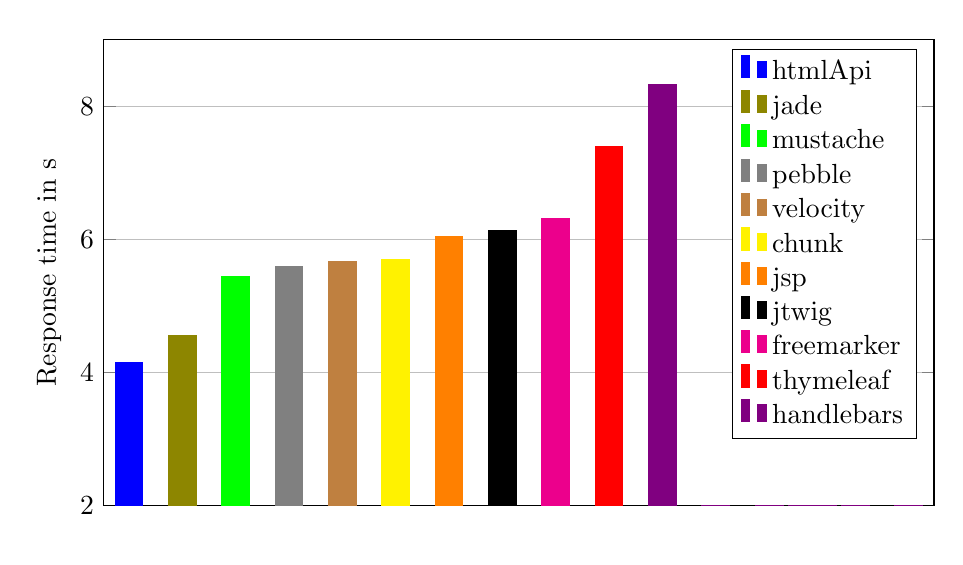
\begin{tikzpicture}
    \begin{axis}[
        width  = 1*\textwidth,
        height = 7.5cm,
        major x tick style = transparent,
        ybar=1*\pgflinewidth,
        bar width=10pt,
        ymajorgrids = true,
        ylabel = {Response time in s},
		symbolic x coords={htmlApi,jade,mustache,pebble,velocity,chunk,jsp,jtwig,freemarker,thymeleaf,handlebars, dummy1, dummy2, dummy3},
        %xtick = data,
        xticklabels = {},
        scaled y ticks = false,
        enlarge x limits=0.8,
        ymin=2,
        ymax=9,
        legend cell align=left,]
                
        \addplot[style={blue,fill=blue,mark=none}]
            coordinates {(htmlApi, 4.151)};
        \addplot[style={olive,fill=olive,mark=none}]
            coordinates {(jade, 4.557)};
        \addplot[style={green,fill=green,mark=none}]
            coordinates {(mustache, 5.448)};
        \addplot[style={gray,fill=gray,mark=none}]
            coordinates {(pebble, 5.588)};
        \addplot[style={brown,fill=brown,mark=none}]
            coordinates {(velocity, 5.672)};
        \addplot[style={yellow,fill=yellow,mark=none}]
            coordinates {(chunk, 5.698)};
        \addplot[style={orange,fill=orange,mark=none}]
            coordinates {(jsp, 6.042)};
        \addplot[style={black,fill=black,mark=none}]
            coordinates {(jtwig, 6.135)};
        \addplot[style={magenta,fill=magenta,mark=none}]
            coordinates {(freemarker, 6.307)};
        \addplot[style={red,fill=red,mark=none}]
            coordinates {(thymeleaf, 7.401)};
        \addplot[style={violet,fill=violet,mark=none}]
            coordinates {(handlebars, 8.323)};
        \addplot[style={violet,fill=violet,mark=none}]
            coordinates {(dummy1, 0)};
        \addplot[style={violet,fill=violet,mark=none}]
            coordinates {(dummy2, 0)};
        \addplot[style={violet,fill=violet,mark=none}]
            coordinates {(dummy3, 0)};
        \addplot[style={violet,fill=violet,mark=none}]
            coordinates {(dummy1, 0)};
        \addplot[style={violet,fill=violet,mark=none}]
            coordinates {(dummy2, 0)};
        \addplot[style={violet,fill=violet,mark=none}]
            coordinates {(dummy3, 0)};
        \legend{htmlApi, jade, mustache, pebble, velocity, chunk, jsp, jtwig, freemarker, thymeleaf, handlebars}
    \end{axis}
\end{tikzpicture}

\newpage

100.000 requests, 10 threads, Spring overhead 9.890 seconds:

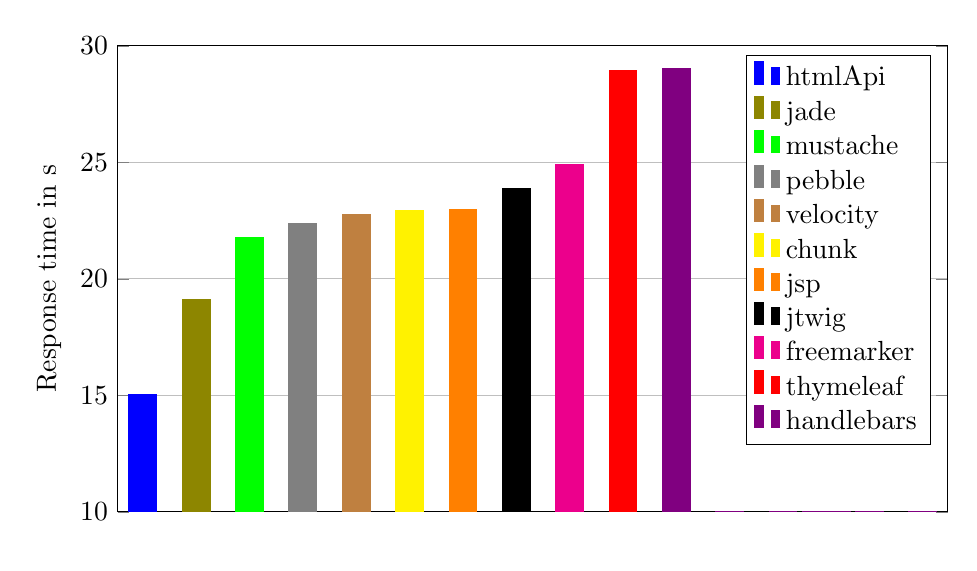
\begin{tikzpicture}
    \begin{axis}[
        width  = 1*\textwidth,
        height = 7.5cm,
        major x tick style = transparent,
        ybar=1*\pgflinewidth,
        bar width=10pt,
        ymajorgrids = true,
        ylabel = {Response time in s},
		symbolic x coords={htmlApi,jade,mustache,pebble,velocity,chunk,jsp,jtwig,freemarker,thymeleaf,handlebars, dummy1, dummy2, dummy3},
        %xtick = data,
        xticklabels = {},
        scaled y ticks = false,
        enlarge x limits=0.8,
        ymin=10,
        ymax=30,
        legend cell align=left,]
                
        \addplot[style={blue,fill=blue,mark=none}]
            coordinates {(htmlApi, 15.049)};
        \addplot[style={olive,fill=olive,mark=none}]
            coordinates {(jade, 19.111)};
        \addplot[style={green,fill=green,mark=none}]
            coordinates {(mustache, 21.783)};
        \addplot[style={gray,fill=gray,mark=none}]
            coordinates {(pebble, 22.377)};
        \addplot[style={brown,fill=brown,mark=none}]
            coordinates {(velocity, 22.763)};
        \addplot[style={yellow,fill=yellow,mark=none}]
            coordinates {(chunk, 22.924)};
        \addplot[style={orange,fill=orange,mark=none}]
            coordinates {(jsp, 22.987)};
        \addplot[style={black,fill=black,mark=none}]
            coordinates {(jtwig, 23.862)};
        \addplot[style={magenta,fill=magenta,mark=none}]
            coordinates {(freemarker, 24.916)};
        \addplot[style={red,fill=red,mark=none}]
            coordinates {(thymeleaf, 28.956)};
        \addplot[style={violet,fill=violet,mark=none}]
            coordinates {(handlebars, 29.034)};
        \addplot[style={violet,fill=violet,mark=none}]
            coordinates {(dummy1, 0)};
        \addplot[style={violet,fill=violet,mark=none}]
            coordinates {(dummy2, 0)};
        \addplot[style={violet,fill=violet,mark=none}]
            coordinates {(dummy3, 0)};
        \addplot[style={violet,fill=violet,mark=none}]
            coordinates {(dummy1, 0)};
        \addplot[style={violet,fill=violet,mark=none}]
            coordinates {(dummy2, 0)};
        \addplot[style={violet,fill=violet,mark=none}]
            coordinates {(dummy3, 0)};
        \legend{htmlApi, jade, mustache, pebble, velocity, chunk, jsp, jtwig, freemarker, thymeleaf, handlebars}
    \end{axis}
\end{tikzpicture}

\noindent
As the results show, HtmlApi outperforms all the template engines in the examples presented with the gap in performance increasing as the number of elements grows. With the two examples presented with 30.000 requests we can observe that the results are approximately the same, even though the concurrent request count increased from 10 to 25, with some template engines performing a bit better and other a bit worse, which may be due to invariable execution variations.

% 10k requests - 10 concurrence
% 
% htmlApi    - 2.578 seconds
% jade       - 2.750 seconds
% mustache   - 3.189 seconds
% pebble     - 3.266 seconds
% velocity   - 3.297 seconds
% chunk      - 3.313 seconds
% jsp        - 3.402 seconds
% jtwig      - 3.406 seconds
% freemarker - 3.438 seconds
% thymeleaf  - 3.781 seconds
% handlebars - 3.922 seconds
% 
% 30k requests - 10 concurrence
% 
% htmlApi    - 7.735 seconds
% jade       - 8.547 seconds
% mustache   - 9.438 seconds
% pebble     - 9.750 seconds
% freemarker - 9.782 seconds
% velocity   - 9.922 seconds
% chunk      - 9.938 seconds
% jsp        - 10.172 seconds
% jtwig      - 10.172 seconds
% thymeleaf  - 11.251 seconds
% handlebars - 11.844 seconds
% 
% 30k requests - 25 concurrence
% 
% htmlApi    - 7.938 seconds
% jade       - 8.344 seconds
% mustache   - 9.235 seconds
% pebble     - 9.375 seconds
% freemarker - 9.459 seconds
% velocity   - 9.485 seconds
% chunk      - 9.829 seconds
% jsp        - 9.922 seconds
% jtwig      - 10.094 seconds
% thymeleaf  - 11.188 seconds
% handlebars - 12.110 seconds
% 
% 
% 100k requests - 10 concurrence
% 
% htmlApi    - 24.939 seconds
% jade       - 29.001 seconds
% mustache   - 31.673 seconds
% pebble     - 32.267 seconds
% freemarker - 32.653 seconds
% chunk      - 32.814 seconds
% velocity   - 32.877 seconds
% jtwig      - 33.752 seconds
% jsp        - 34.806 seconds
% thymeleaf  - 38.846 seconds
% handlebars - 38.924 seconds

